\chapter{Application infrastructure and architecture}

In this chapter I am going to talk about the services that \textbf{Think-In} relies on and why I chose them, afterwards I am going to talk about the application's architecture, used technologies and tools.

\section{Application infrastructure}

\textbf{Think-In} is supposed to be an application with people networking in mind, therefore allowing humans far away from each other to connect. Because of this, it had to be available to the public internet. Hosting the application on my own machine would have implied a lot of time spent on maintenance, implementation and let's not even mention the security nightmare that it would have been. The issue of scalability would have been impossible to solve as well. Quickly thereafter I realised that XaaS\footnote{Everything as a service: \href{https://en.wikipedia.org/wiki/As\_a\_service}{https://en.wikipedia.org/wiki/As\_a\_service}} offerings by cloud computing providers would solve the issues I would face and it would save a lot of time and energy, all while using robust and proven to work software.

\subsection{Choosing a main cloud platform to use}

During my research I have found Gartner\footnote{Research and advisory firm: \href{https://www.gartner.com/en}{https://www.gartner.com/en}} to have a great reputation and provide reliable reports on cloud computing service providers. As a result I chose to inspect their famous magic quadrants during which I have found a \textit{Magic Quadrant for Cloud Infrastructure and Platform Services}\footnote{\href{https://aws.amazon.com/blogs/aws/aws-named-as-a-cloud-leader-for-the-10th-consecutive-year-in-gartners-infrastructure-platform-services-magic-quadrant/}{https://aws.amazon.com/blogs/aws/aws-named-as-a-cloud-leader-for-the-10th-consecutive-year-in-gartners-infrastructure-platform-services-magic-quadrant/}}. Instinctively I would choose a provider with significant age in the field because if I were to face an issue then certainly I wouldn't be first one to do so and I would easily find a fix on the web. Moreover I would expect a cloud provider with experience to have well written documentation about their services, which, because I am a beginner, is essential to me. As a consequence I will consider only the very well known providers as an option.

In the top right quadrant for this specific report (corresponding to the leaders in this domain) I found three providers: Google, Microsoft and Amazon Web Services. All of them have a free offering so I went to research by using each one individually:

\begin{description}[style=unboxed, labelwidth=\linewidth]
	\item[Google Cloud Platform]
	Out of all three providers I found Google to have the best project organization, all created resources are within a logical entity (a project) and that would help me as a newcomer to not confuse resources. Moreover they have the most generous free tier. Unfortunately I found certain services not to work as good as others, for example their API Gateway seems to lack in features compared to the one provided by AWS, it was also hard to read event logs from Cloud Functions.
    \item[Microsoft Azure]
	I have found this platform to be more confusing than others, I also did not like the experience using the web console (e.g. horizontal scrolling), more than this I had trouble using the web console to upload a collection of files under a directory on their object storage service.
	\item[Amazon Web Services (AWS)]
	I "clicked" with the services provided by AWS more than any other cloud provider, they felt simple to use and packed with features. AWS has been available for more time than the other two and is very well established which for sure meant great documentation and lots of resources to learn from. One thing I found inferior compared to others was the organization of resources based on regions.
\end{description}

This being said, I chose Amazon Web Services as the main cloud provider.

\section{Application architecture}

Below is attached a simplified overview of the application's architecture, it can be used as a reference when we will go into more detail about the implementation.

\begin{figure}[H]
	\centering
	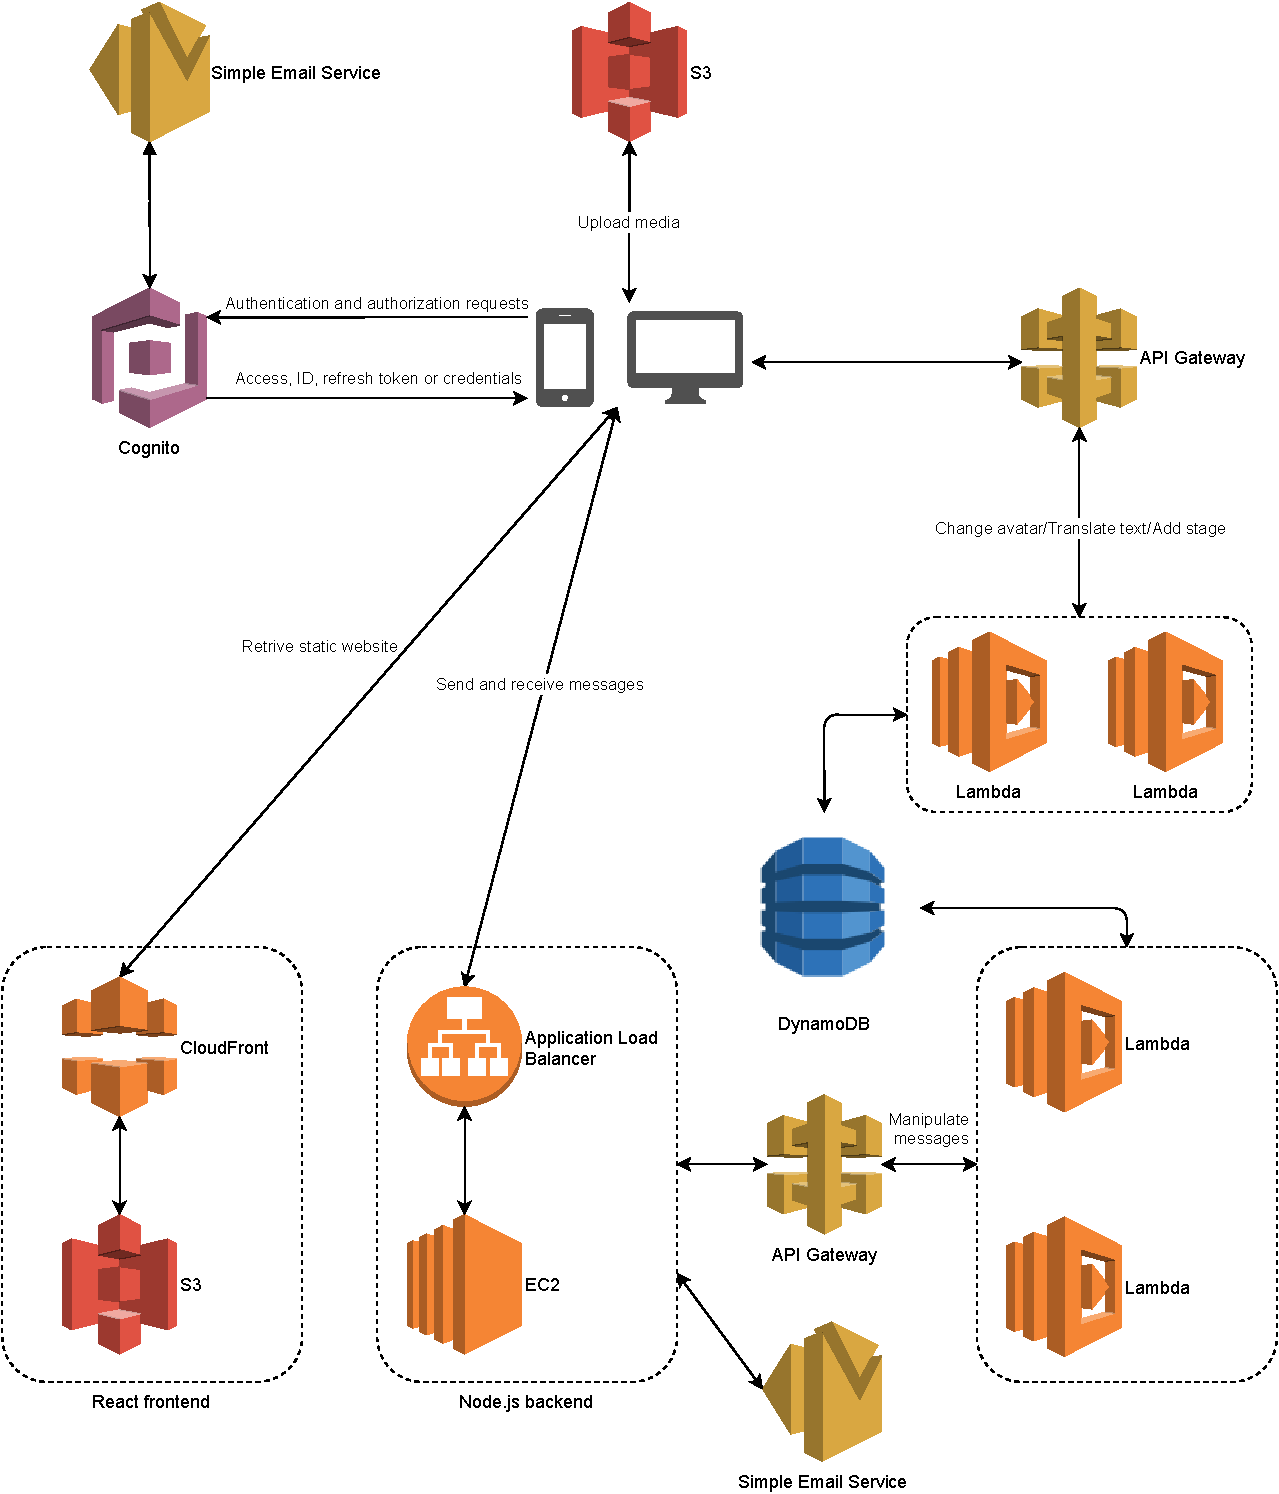
\includegraphics[width=\textwidth,keepaspectratio]{images/architecture/architecture.pdf}
	\caption{Application architecture.}
	\label{figure:application-architecture}
\end{figure}

Efforts were put into making the application scale as well as possible, this is why for instance the REST API was created from HTTP triggered Lambda functions, they scale to "infinity". Interesting aspects are that the API is accessed both client-side and server-side, everything that could be done from the client has been done from the client, however as we will see later some actions are only possible on the backend. The backend performs communication using websockets in order to ensure real-time message transmission.

Instead of creating an authentication system I relied that weight on AWS Cognito user pools\footnote{\href{https://docs.aws.amazon.com/cognito/latest/developerguide/cognito-user-identity-pools.html}{https://docs.aws.amazon.com/cognito/latest/developerguide/cognito-user-identity-pools.html}} so that I could easily manage user confirmation, password resets, changing email or other attributes and more without having to build that infrastructure myself. Moreover, Cognito was also used for providing temporary AWS credentials for certain services (e.g S3) so that the client could interact with these services directly.

\section{Continuous Integration and Continuous Deployment}

As talked about in the last chapter, values were found in having short and quick releases, therefore a pipeline that automates the process of deploying the application was set up. Below, in Figure \ref{figure:cicd}, is a diagram showcasing the flow of how the application is built.

\begin{figure}[H]
	\centering
	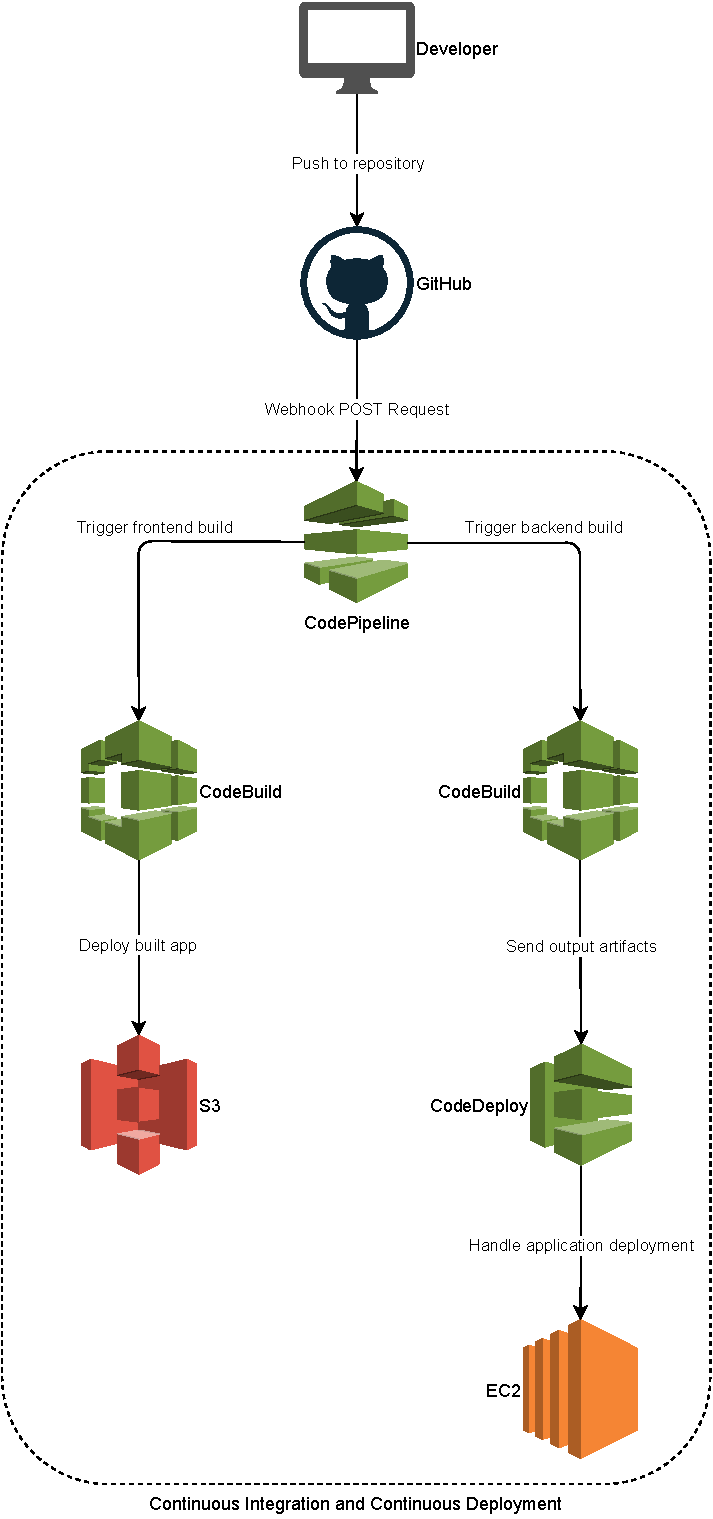
\includegraphics[width=.7\textwidth,keepaspectratio]{images/architecture/cicd.pdf}
	\caption{Continuous Integration and Continuous Deployment overview.}
	\label{figure:cicd}
\end{figure}

For those more familiar with CodePipeline, a screenshot of the pipeline from the AWS console is shown in Figure \ref{figure:codepipeline-cicd}.

\begin{figure}[H]
	\centering
	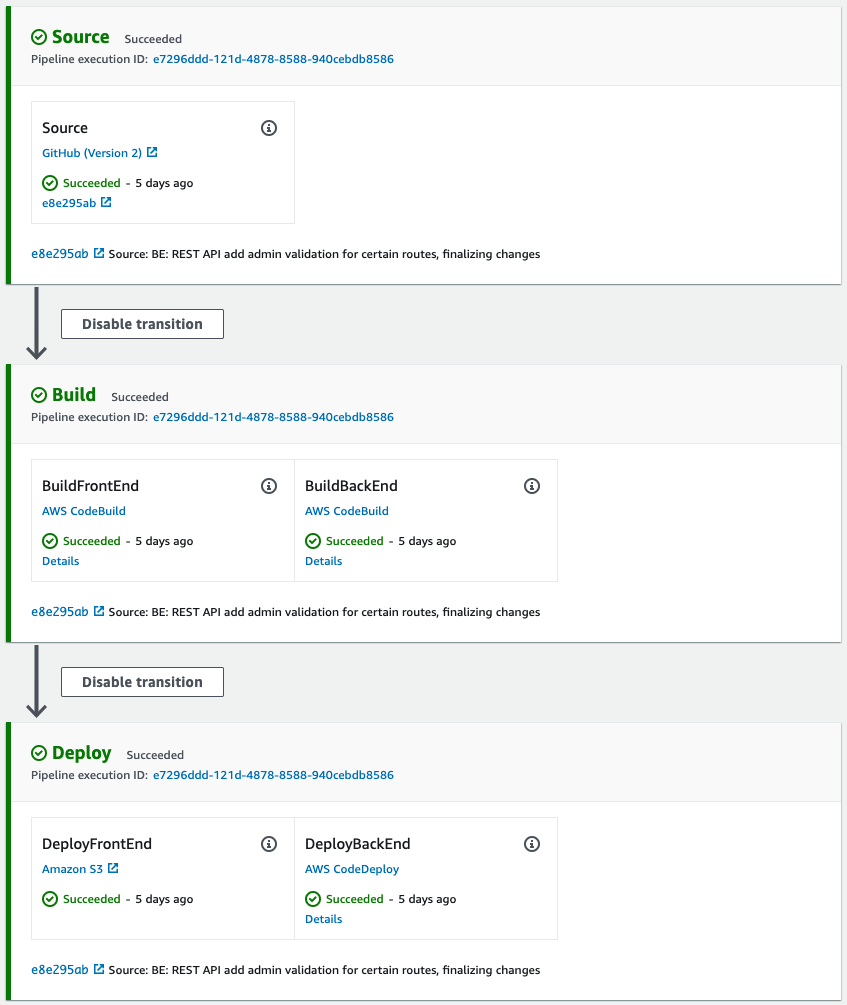
\includegraphics[width=\textwidth,keepaspectratio]{images/architecture/codepipeline-cicd.png}
	\caption{CodePipeline from AWS console.}
	\label{figure:codepipeline-cicd}
\end{figure}

Whenever a push to the GitHub repository is done, a webhook is triggered and GitHub sends a POST request to AWS that starts the pipeline. I set up the pipeline so that two parallel builds are started at once: the \textbf{frontend} and \textbf{backend} builds.

The code executed for the frontend build can be found in Figure \ref{figure:cicd-frontend-buildspec}. In the \textit{install} phase the npm\footnote{\href{https://www.npmjs.com/}{https://www.npmjs.com/}} package manager is installed in a non-interactive way (as a result of the \verb|--assume-yes| option) which is needed for installing the application's dependencies. Because all the source code is organized into a monorepo\footnote{\href{https://en.wikipedia.org/wiki/Monorepo}{https://en.wikipedia.org/wiki/Monorepo}}, in the \textit{pre\_build} phase the working directory has to be changed, in this case to the directory where the frontend application is. Next, on line 14, a clean install of the application's dependencies is done. In the \textit{build} phase I have abstracted the exporting of the application in a single npm script. After the \textit{build} phase is done, the output artifacts corresponding to the built application are put into a S3 bucket from where the CloudFront CDN will serve the static files to clients.

\begin{figure}[H]
\begin{lstlisting}[numbers=left,language=yaml]
version: 0.2
phases:
  install:
    runtime-versions:
      nodejs: 14.x
    commands:
      - apt --assume-yes update
      - apt --assume-yes install npm
    finally:
      - echo Install phase done.
  pre_build:
    commands:
      - cd app/FE
      - npm ci
    finally:
      - echo Prebuild phase done.
  build:
    commands:
      - npm run export
    finally:
      - echo Build phase done.
artifacts:
  base-directory: 'app/FE/out'
  files:
    - '**/*'
\end{lstlisting}
\caption{Frontend CodeBuild specification}
\label{figure:cicd-frontend-buildspec}
\end{figure}

On the other side, the code executed by CodeBuild for the backend build can be found in Figure \ref{figure:cicd-backend-buildspec}. The \textit{install} phase is the same as in the frontend build specification. Similar to the frontend, in the \textit{pre\_build} phase we change the working directory to where the backend app is and install the dependencies. The first command in the \textit{build} phase creates the environment file on the fly by retrieving the environment variables I have stored in AWS System Manager Parameter Store\footnote{Centralized place for keeping secrets/parameters: \href{https://aws.amazon.com/systems-manager/}{https://aws.amazon.com/systems-manager/}}. The next command builds the application, after which the output artifacts are passed on to CodeDeploy.

\begin{figure}[H]
\begin{lstlisting}[numbers=left,language=yaml]
version: 0.2
phases:
  install:
    runtime-versions:
      nodejs: 14.x
    commands:
      - apt --assume-yes update
      - apt --assume-yes install npm
    finally:
      - echo Install phase done.
  pre_build:
    commands:
      - cd app/BE/stage_server
      - npm ci
    finally:
      - echo Prebuild phase done.
  build:
    commands:
      - npm run create-env
      - npm run build
    finally:
      - echo Build phase done.
artifacts:
  base-directory: 'app/BE/stage_server'
  exclude-paths: 'src/**/*'
  files: '**/*'
\end{lstlisting}
\caption{Backend CodeBuild specification}
\label{figure:cicd-backend-buildspec}
\end{figure}

The artifacts are now in CodeDeploy's hands which has the specification shown in Figure \ref{figure:cicd-backend-appspec}. Lines 3-5 specify the path to where the artifacts will be put on the EC2 machine. Lines 7-12 attach shell scripts to different lifecycle events which are self-explanatory, now we will explore each script in detail.

\begin{figure}[H]
\begin{lstlisting}[numbers=left,language=yaml]
version: 0.0
os: linux
files:
  - source: /
    destination: /home/ubuntu/websocket-server/
hooks:
  ApplicationStop:
    - location: ./scripts/application-stop.sh
  BeforeInstall:
    - location: ./scripts/before-install.sh
  ApplicationStart:
    - location: ./scripts/application-start.sh
\end{lstlisting}
\caption{Backend CodeDeploy specification}
\label{figure:cicd-backend-appspec}
\end{figure}

The \textit{application-stop.sh} script (Figure \ref{figure:cicd-backend-appspec-application-stop}) is run for the \textit{ApplicationStop} lifecycle event, here we have to stop the previously running application. We store the process id of the running process in the \textit{pid} variable after which, if there was a process id found, the process is killed. Otherwise, corresponding to the case where there is no process id found, nothing happens.

\begin{figure}[H]
\begin{lstlisting}[numbers=left,language=bash]
#!/bin/bash
pid=`ps aux | grep "node out/index.js" | grep -v grep | tr -s " " " "
 | cut -d " " -f2`
# if string is not empty
if [ -n "${pid}" ]
then
    kill -9 $pid
    echo Killed process with pid $pid
else
    echo Found no process with pid $pid
fi
\end{lstlisting}
\caption{Backend CodeDeploy application stop script.}
\label{figure:cicd-backend-appspec-application-stop}
\end{figure}

Next up is the \textit{before-install.sh} script (Figure \ref{figure:cicd-backend-appspec-before-install}). This script simply clears the directory where the application is.

\begin{figure}[H]
\begin{lstlisting}[numbers=left,language=bash]
#!/bin/bash
rm -rf /home/ubuntu/websocket-server
mkdir /home/ubuntu/websocket-server
\end{lstlisting}
\caption{Backend CodeDeploy before install script.}
\label{figure:cicd-backend-appspec-before-install}
\end{figure}

Before this script is ran, the built files have been copied to the \textit{/home/ubuntu/websocket-server} directory. Finally we have the \textit{application-start.sh} script (Figure \ref{figure:cicd-backend-appspec-application-start}). We first navigate to the directory where the application is, we install its dependencies non-interactively and we create the environment file on the fly just like in the build phase. After this everything has been finished and we can start the application by running \textit{yarn start} which corresponds to the command below:

\begin{lstlisting}[language=bash]
nohup node out/index.js > stdout.log 2> stderr.log < /dev/null &
\end{lstlisting}

\begin{figure}[H]
\begin{lstlisting}[numbers=left,language=bash]
#!/bin/bash
cd /home/ubuntu/websocket-server
yarn install --non-interactive
node `dirname "$BASH_SOURCE"`/application-start-create-env.js
yarn start
\end{lstlisting}
\caption{Backend CodeDeploy application start script.}
\label{figure:cicd-backend-appspec-application-start}
\end{figure}

\section{REST API Deployment}

For managing the deployment of the REST API I have relied on Serverless\footnote{\href{https://www.serverless.com/}{https://www.serverless.com/}} framework, it has allowed me to easily deploy AWS resources such as Lambda functions, API Gateway and DynamoDB\footnote{Fast and flexible NoSQL database: \href{https://aws.amazon.com/dynamodb/}{https://aws.amazon.com/dynamodb/}}. For this I have used DevOps practices such as Infrastructure as Code for configuring the resources that are created.

Going further we're going to analyze the configuration code (Figure \ref{figure:iac-function-example}) for a Lambda function as an example. On line 2, we specify the path to the function that will be executed when this Lambda function is triggered. Line 4 to 11 indicate that this function is HTTP triggered whenever a \verb|GET| request is sent to \verb|/chats/{chatId}|, moreover it attaches an authorizer so only tokens created by AWS Cognito are approved. Lines 12-17 define the roles this function has, in this case it allows the \verb|dynamodb:Query| action only on a specific DynamoDB table. As observed I have tried to respect the least privilege principle.

\begin{figure}[H]
\begin{lstlisting}[numbers=left,language=yaml]
get-chats:
    handler: chats/get-chats.getChats
    events:
      - http:
          path: /chats/{chatId}
          method: get
          cors: true
          authorizer:
            type: COGNITO_USER_POOLS
            authorizerId:
              Ref: thinkInApiGatewayAuthorizer
    iamRoleStatements:
      - Effect: 'Allow'
        Action:
          - dynamodb:Query
        Resource: arn:aws:dynamodb:${self:provider.region}:*:table/
        ${self:provider.environment.DYNAMODB_TABLE_NAME}
\end{lstlisting}
\caption{Example of configuration code for a Lambda function.}
\label{figure:iac-function-example}
\end{figure}